\documentclass{beamer}
\usetheme{Madrid}
\beamertemplatenavigationsymbolsempty
\setbeamertemplate{blocks}[rounded][shadow=true]

\usepackage{listings}

\usepackage{amssymb}
\usepackage{amsmath}

\definecolor{mygreen}{rgb}{0,0.6,0}

\lstset{
  basicstyle=\footnotesize,
  breakatwhitespace=false,
  breaklines=false,
  captionpos=b,
  commentstyle=\color{blue},
  extendedchars=true,
  keepspaces=true,
  keywordstyle=\color{mygreen},
  language=Fortran,
  numbers=left,
  numbersep=2pt,
  numberstyle=\tiny\color{gray},
  rulecolor=\color{black},
  showspaces=false,
  showstringspaces=false,
  showtabs=false,
  stepnumber=1,
  tabsize=2,
  title=\lstname
}

\usepackage{setspace}
\setstretch{1.5}

\title{Fortran Standard Library}
\author[]{Jeremie Vandenplas\\[3mm]
Bálint Aradi,
Izaak Beekman,
Ondrej Certik,
Milan Curcic,
Pierre de Buyl,
Juan Fiol,
Michael Hirsch,
Ivan Pribec,
Nathaniel Shaffer}
\date{July 2, 2020}

\begin{document}
\begin{frame}[t]
	\titlepage
\end{frame}	

\begin{frame}[c]{Fortran Standard}
	\begin{itemize}
		\item Published by the International Organization for Standardization (ISO)
		\item Limited set of intrinsic procedures
		\item Possibility to add new intrinsic procedures and modules
		\begin{itemize}
			\item After standardization and implementation in compilers
		\end{itemize}
		\item No Standard Library
	\end{itemize}
	\center
	\textcolor{red}{\textbf{Consequence: we all reinvent the wheel continuously!}}
\end{frame}


\begin{frame}[c]{Aim}
	\center
	\Large
	\textcolor{blue}{Develop} and \textcolor{blue}{provide}\\
	a \textcolor{blue}{community} driven and agreed upon de facto\\
	\textcolor{blue}{standard library}\\
	for Modern Fortran
\end{frame}


\begin{frame}[c]{Fortran Standard Library - stdlib}
	\Large
	\begin{itemize}
		\item One of the four pillars of \textcolor{blue}{fortran-lang}
		\item \textcolor{blue}{MIT} License
		\item GitHub: https://github.com/fortran-lang/stdlib
		\item API docs: https://stdlib.fortran-lang.org
	\end{itemize}
\end{frame}


\begin{frame}[t]{General scope}
	Similar to \textcolor{blue}{SciPy} or
	to the default built-in \textcolor{blue}{Matlab scientific environment}

        \textcolor{mygreen}{Three} topics
	\begin{itemize}
		\item \textcolor{blue}{Algorithms}
		\begin{itemize}
			\item Merging, searching, sorting, ...
		\end{itemize}
		\item \textcolor{blue}{Mathematics}
		\begin{itemize}
			\item Linear algebra, sparse matrices, special functions, fast Fourier transform, random numbers, statistics, ordinary differential equations, numerical integration, optimization, ...
		\end{itemize}
		\item \textcolor{blue}{Utilities}
		\begin{itemize}
			\item Containers, strings, files, OS/environment integration, unit testing, assertions, logging, ...
		\end{itemize}
	\end{itemize}
\end{frame}


\begin{frame}[c]{Currently implemented in stdlib}
	\begin{block}{~\vspace{0.5cm}}
	\vspace{-0.8cm}
	\begin{tabular}{ccc}
		\textcolor{white}{\bf Module} &\textcolor{white}{\bf Description} &\textcolor{white}{\bf \# procedures} \\
		ascii & & 16\\
		error & Catching and handling errors & 2\\
		io & Input/output helper and convenience & 3\\
		kinds & & -\\
		linalg & Linear algebra & 3\\
		optval & Fallback value for optional arguments & 1\\
		quadrature & Numerical integration & 4\\
		stats & Descriptive statistics & 5\\
		system & & 1 \\
	\end{tabular}
	\end{block}
\end{frame}


\begin{frame}[fragile]{Examples}
	\begin{lstlisting}
	...
	use stdlib_experimental_io, only: loadtxt, savetxt
	use stdlib_experimental_linalg, only: diag
	use stdlib_experimental_stats, only: moment
	...
	real, allocatable :: A(:,:)
	call loadtxt('example.dat', A)
	...
	print*, diag(A)
	...
 	call savetxt('moment.dat',&
	  moment(A, order = 3, dim = 1, mask = (A > 5.)))
	...	\end{lstlisting}
\end{frame}


\begin{frame}[fragile]{Example - optval}
	\begin{lstlisting}
	...
	use  stdlib_experimental_optval, only: optval
	...
	real function root(x, n)
	  real, intent(in) :: x
	  integer, intent(in), optional :: n
	  root = x**(1.0/optval(n, 2))
	end function
	\end{lstlisting}
\end{frame}


\begin{frame}[c]{API docs (https://stdlib.fortran-lang.org)}
	\begin{center}
	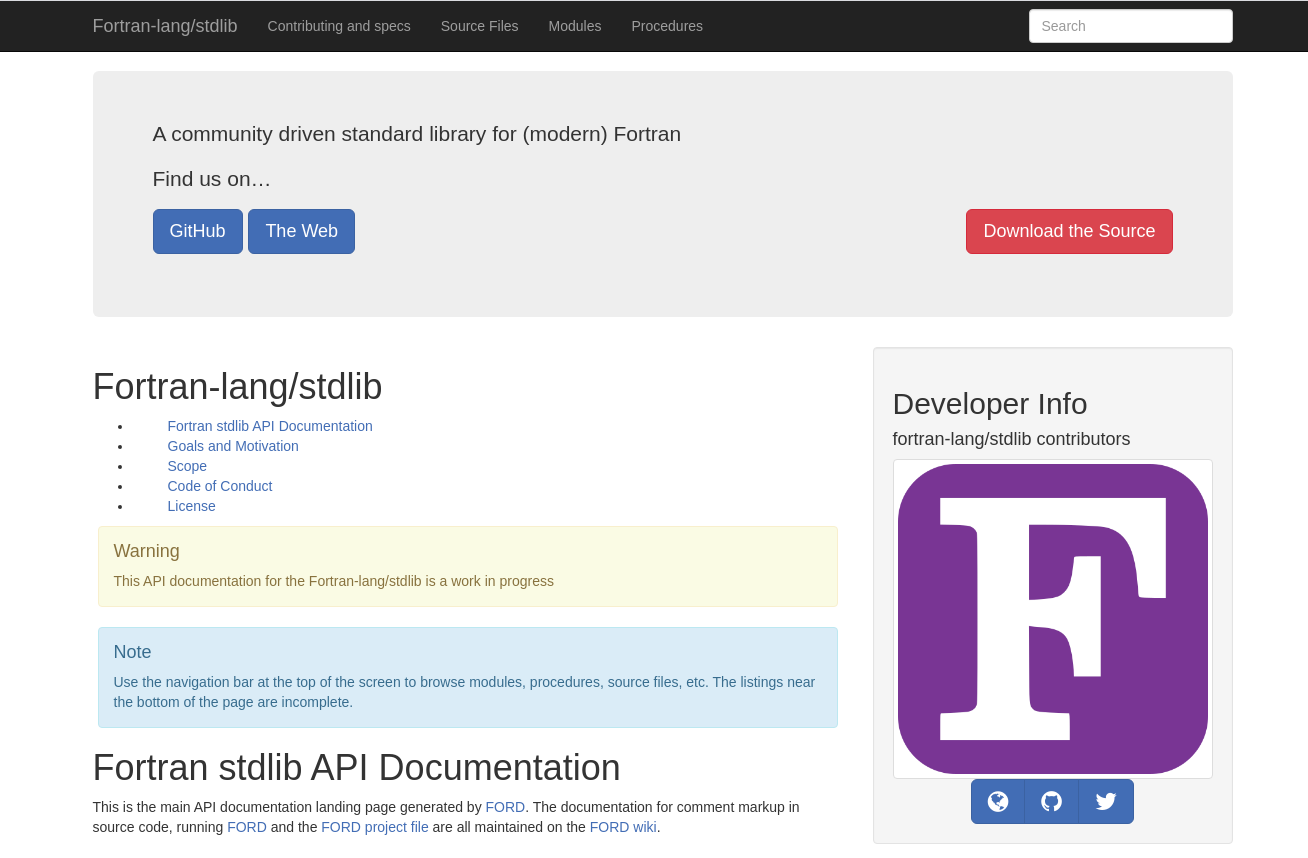
\includegraphics[width=0.9\textwidth]{apidocsstdlib}
	\end{center}
\end{frame}


\begin{frame}[c]{API docs (https://stdlib.fortran-lang.org)}
	Automatically generated by \textcolor{blue}{FORD} %https://github.com/Fortran-FOSS-Programmers/ford
	\begin{itemize}
		\item Source codes
		\item \textcolor{blue}{Markdown specs} for all procedures
		\begin{itemize}
			\item \textit{Description}
			\item \textit{Syntax}
			\item \textit{Arguments}
			\item \textit{Output} / \textit{Return value}
			\item \textit{Example}
		\end{itemize}
	\end{itemize}

\end{frame}


\begin{frame}[c]{Contributions through GitHub}
	https://github.com/fortran-lang/stdlib\\
	\textcolor{blue}{Source codes}
	\begin{itemize}
		\item 16 contributors
		\item $>$ 100 Pull Requests
	\end{itemize}
	\textcolor{blue}{Issues / ideas / comments}
	\begin{itemize}
		\item 47 contributors
		\item $>$ 110 GitHub issues
	\end{itemize}	
\end{frame}


\begin{frame}[c]{How to contribute to stdlib?}
	\textcolor{blue}{Through GitHub}\\
	\begin{itemize}
		\item Issues
		\begin{itemize}
			\item Proposition of ideas, issues, comments
		\end{itemize}
		\item Pull Requests
		\begin{itemize}
			\item To contribute to the source code and specs
		\end{itemize}
	\end{itemize}
	\textcolor{blue}{Code of Conduct}\\
\end{frame}

\begin{frame}[c]{Contributing to the source code?}
	\textcolor{blue}{Workflow}
	\begin{enumerate}
		\item Proposition of an \textbf{idea}
		\item Proposition of the \textbf{API}
		\item Discussion of the \textbf{specs}
		\item Pull request of an \textbf{implementation} in the experimental namespace + associated unit tests
		\item Stable \textbf{release} of procedures in the experimental namespace
	\end{enumerate}
\end{frame}


\begin{frame}[c]{Acknowledgments}
	
\end{frame}

\begin{frame}[c]{}
	\centering \Huge
	\emph{Thank you!}
\end{frame}

\end{document}
